\documentclass[12pt]{article}
\usepackage[margin = 2.4cm]{geometry} % For margins of 3cm
\usepackage{graphicx}
\usepackage{float} % For H float position
\usepackage{gensymb} % For some symbols
\usepackage{amsfonts, amssymb, amsmath} % All three for maths symbols
\usepackage[export]{adjustbox} % For figure frames
\setlength{\parskip}{6pt} % To make nice looking paragraph spacing
\usepackage[export]{adjustbox} % For figure frames
\usepackage{rotating}
\usepackage[section]{placeins}
\usepackage{setspace} % For double spacing
\usepackage{pdfpages} % Allows including PDFs
\usepackage[sort&compress]{natbib} % bibliographies
\doublespacing
\usepackage{titling}
\newcommand{\subtitle}[1]{%
	\posttitle{%
		\par
	\end{center}
    \begin{center}\large#1\end{center}
    \vskip0.5em}
}

\title{Effect of DHODH mutation on p53 expression and osteoblast differentiation}
\author{Urwah Nawaz \\ a1654797}
\subtitle{\textbf{Preliminary RHEP} \\Word Count: 574}

\date{}
\begin{document}
	\maketitle
\paragraph{Declaration:}
~\\This work does not contain any material written by another person, except where due reference is given in the text, and the work has not been presented previously as a component of any other academic course.	
 
 \pagebreak

	\section{Background}
Miller's syndrome (MS) is a rare autosomal disorder characterised by craniofacial and postaxial limb deformities \citep{miller1979postaxial}.  The gene \textit{DHODH} encodes dihydroorotate dehydrogenase (DHODH); mutations in this gene have been implicated in MS and results in DHODH loss-of-function (LOF) \citep{ng2010exome, doi:10.1093/hmg/dds218}. DHODH is a key enzyme in the \textit{de novo} pyrimidine synthesis pathway, and links it the mitochondrial respiratory chain (MRC) \citep{fang2013dihydro}. The mechanisms by which \textit{DHODH} mutation results in MS phenotype are not fully understood. 

DHODH inhibition causes impairment of pyrimidine synthesis, and mitochondrial dysfunction. In both cases DHODH inhibition has demonstrated a contribution to p53 stabilization  \citep{linke1996reversible, khutornenko2010pyrimidine, fairus2017dihydroorotate}. Analysis of \textit{Dhodh} expression in mouse embryo showed spatio-temporal specific activity in pharyngeal arches and limb-buds, precursors to tissues affected in MS \citep{doi:10.1093/hmg/dds218} indicating DHODH mutation may specifically affect the embryo. The effect of p53 has been explored in Treacher-Collins syndrome (TCS), another craniofacial disorder. Trp53 knock-out in TCS mouse models ameliorated the craniofacial anomalies showing that p53 plays a role TCS pathology \citep{jones2008prevention}. Trp53 levels were linked to increased endogenous ROS production \citep{sakai2016prevention}. These observations indicate that p53 over-expression in embryo leads to craniofacial abnormalities. \textit{DHODH} mutations may cause p53 up-regulation either via pyrimidine deficiency, mitochondrial dysfunction or in combination during embryonic development. 


%Impairment of pyrimidine synthesis has been linked to p53 activation due to nucleotide starvation, and has been implicated in MS pathology \citep{linke1996reversible}. \textit{Dhodh} expression in mouse embryo showed spatio-temporal specific activity in pharyngeal arches and limb-buds. These are all precursors to tissues affected in MS \citep{doi:10.1093/hmg/dds218}. Thus DHODH mutation may specifically affect the embryo.  p53 levels also show increase due to mitochondrial function caused by DHODH inhibition. DHODH inhibition leads to increase in endogenous reactive oxygen species (ROS) production causing oxidative stress and p53 stabilization \citep{khutornenko2010pyrimidine, fairus2017dihydroorotate}.  \textit{Trp}53 knock-out in mouse model embryos of Treacher-Collins syndrome (TCS), another craniofacial disorder,  ameliorated the craniofacial anomalies showing that p53 plays a role TCS pathology  \citep{jones2008prevention}. High levels of \textit{Trp}53 were linked to increased endogenous ROS production \citep{sakai2016prevention}. These observations connect p53 over-expression in embryo to craniofacial abnormalities. This suggests that \textit{DHODH} mutations may work in a similar manner either via pyrimidine deficiency, mitochondrial dysfunction or in combination . 

The primary phenotype associated with MS diagnosis is craniofacial and limb skeleton abnormalities. MC3T3-E1 cells have been used to show that depletion of DHODH decreased osteogenic gene expression \citep{fang2016dihydroorotate}. While p53 levels showed an increase in this study, its relation to osteoblast differentiation was not explored. MC3T3-E1 cells contains Osterix/SP7, a transcription factor required for proper osteoblast differentiation \citep{tian2012osterix}. Conditional inactivation of Osx/SP7 in cranial neural crest cells of mice has shown defects in craniofacial bone development \citep{baek2013osterix}. Additionally, a human patient with a homozygous mutation in Osx/SP7 displayed craniofacial and limb bone deformities suggesting roles of Osx/SP7 in bone differentiation and patterning during embryonic development \citep{lapunzina2010identification}.  p53 is able to exert a repressive effect on  Osx/SP7 leading to inhibition of osteoblast differentiation \citep{p53sp7}.  \textit{Osx} mRNA levels show significant up-regulation between E11.5 and E13.5 during mouse embryonic development, subsequent to the increased \textit{Dhodh} expression observed at E10.5 \citep{ gao2004molecular,  kaback2008osterix, doi:10.1093/hmg/dds218}. Therefore one of the mechanisms by which \textit{DHODH} mutation causes the MS phenotype is by inhibiting  Osx/SP7  due to p53 over-expression during craniofacial and limb development. 


\section{Hypothesis, Aims and Experiment}	
\textbf{Hypothesis}: \textit{DHODH} gene mutation causes stabilization of p53 in the embryo leading to disrupted osteoblast differentiation and bone hypoplasia by inhibiting Osterix/SP7 in Miller's syndrome.
\begin{itemize}
	\item {\textbf{Aim 1}}: To check if DHODH LOF is causing p53 stabilization in the developing embryo.
	\item {\textbf{Aim 2}}: To confirm if Osx/SP7 expression during craniofacial and limb development are affected by DHODH LOF due to p53 stabilization
	\item {\textbf{Aim 3}}: To understand the pathway that causes p53 stabilization due to DHODH LOF 
\end{itemize}


\paragraph{Mouse Model}:
\\ 
MS mouse model generation and other controls have been summarised in Table 1. 

\begin{table}[!htp]
	\centering
	\footnotesize
	\caption{Mice and controls for this experiment}
	\label{my-label}
	\begin{tabular}{lll}
		Controls                                                                                                  & Generated using                                                                                                                                                                                                                                                                               & Group                    \\ \hline
		\multicolumn{1}{|l|}{Wildtype mouse (WT)}                                                                 & \multicolumn{1}{l|}{C57BL/6 wild type mouse}                                                                                                                                                                                                                                                  & \multicolumn{1}{l|}{I} \\ \hline
		\multicolumn{1}{|l|}{Dhodh(-/-) LOF mice}                                                                 & \multicolumn{1}{l|}{\begin{tabular}[c]{@{}l@{}}CRISPR-Cas9 can be used to specifically mutate the locus of\\ mouse ortholog of DHODH to generate the same  LOF alleles \\ found Millers patients 
				as described in \cite{qin2016generating} \\ CRISPR-Cas9 makes it easier to generate mouse models \\ of any background.\end{tabular}} & \multicolumn{1}{l|}{II} \\ \hline
		\multicolumn{1}{|l|}{\begin{tabular}[c]{@{}l@{}}Trp53+/- mice on a \\ C57BL/6 background\end{tabular}}     & \multicolumn{1}{l|}{Generated as previously described by \cite{jones2008prevention}}                                                                                                                                                                                                                                         & \multicolumn{1}{l|}{III} \\ \hline
		\multicolumn{1}{|l|}{\begin{tabular}[c]{@{}l@{}}Trp53+/- mixed with\\  Dhodh(-/-) LOF mice\end{tabular}}  & \multicolumn{1}{l|}{\begin{tabular}[c]{@{}l@{}}The Trp53+/- mice on a C57BL/6 background will be\\  bred with Dhodh(-/-) LOF mice as described by \cite{jones2008prevention} \\ for TCS mouse model \end{tabular}}                                                                                                                   & \multicolumn{1}{l|}{IV} \\ \hline
		\multicolumn{1}{|l|}{\begin{tabular}[c]{@{}l@{}}WT mouse treated with\\ leflunomide\end{tabular}}         & \multicolumn{1}{l|}{Leflunomide (LFN) is a known inhibitor for DHODH}                                                                                                                                                                                                                               & \multicolumn{1}{l|}{V} \\ \hline
	\end{tabular}
\end{table}



A skeletal analysis should be performed on E17.5 embryos to ensure that craniofacial and limb abnormalities are observed for MS model. Immunoblotting will confirm low DHODH levels in the model, described previously by \cite{sakai2016prevention} for TCS mouse model.                                                                                                                              



\textbf{Experiment Plan}


	\begin{figure}[!htp]
		\centering
	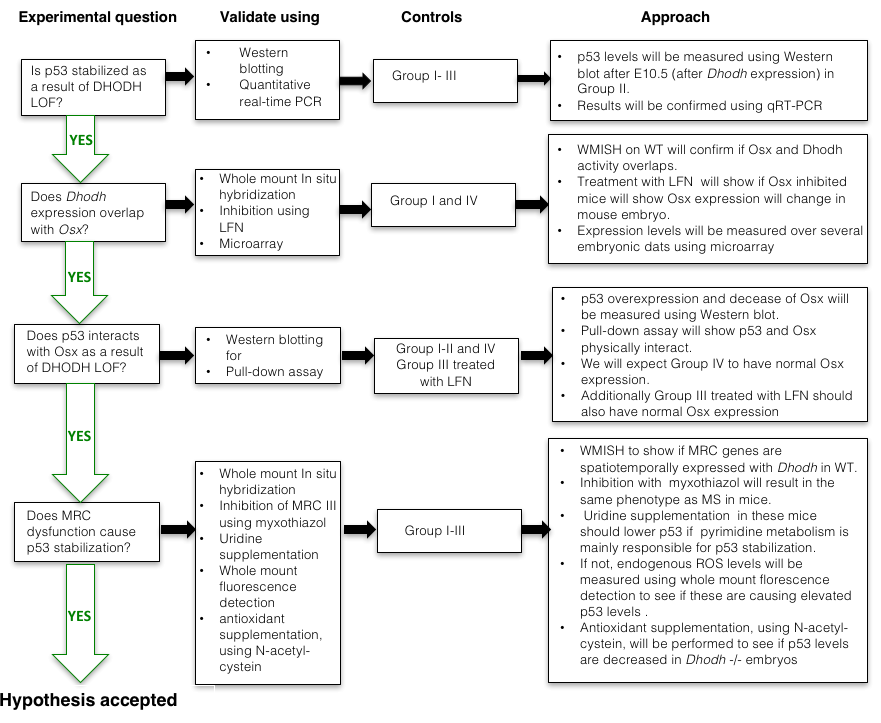
\includegraphics[width=1.10\linewidth]{Figures/plan1}
	\caption{Experimental plan. Green arrow indicates expected results from experiments. For Control groups, refer to Table 1}
	\label{fig:plan2}
	\end{figure}
	
\pagebreak

\bibliography{references/references.bib}
\bibliographystyle{apa}


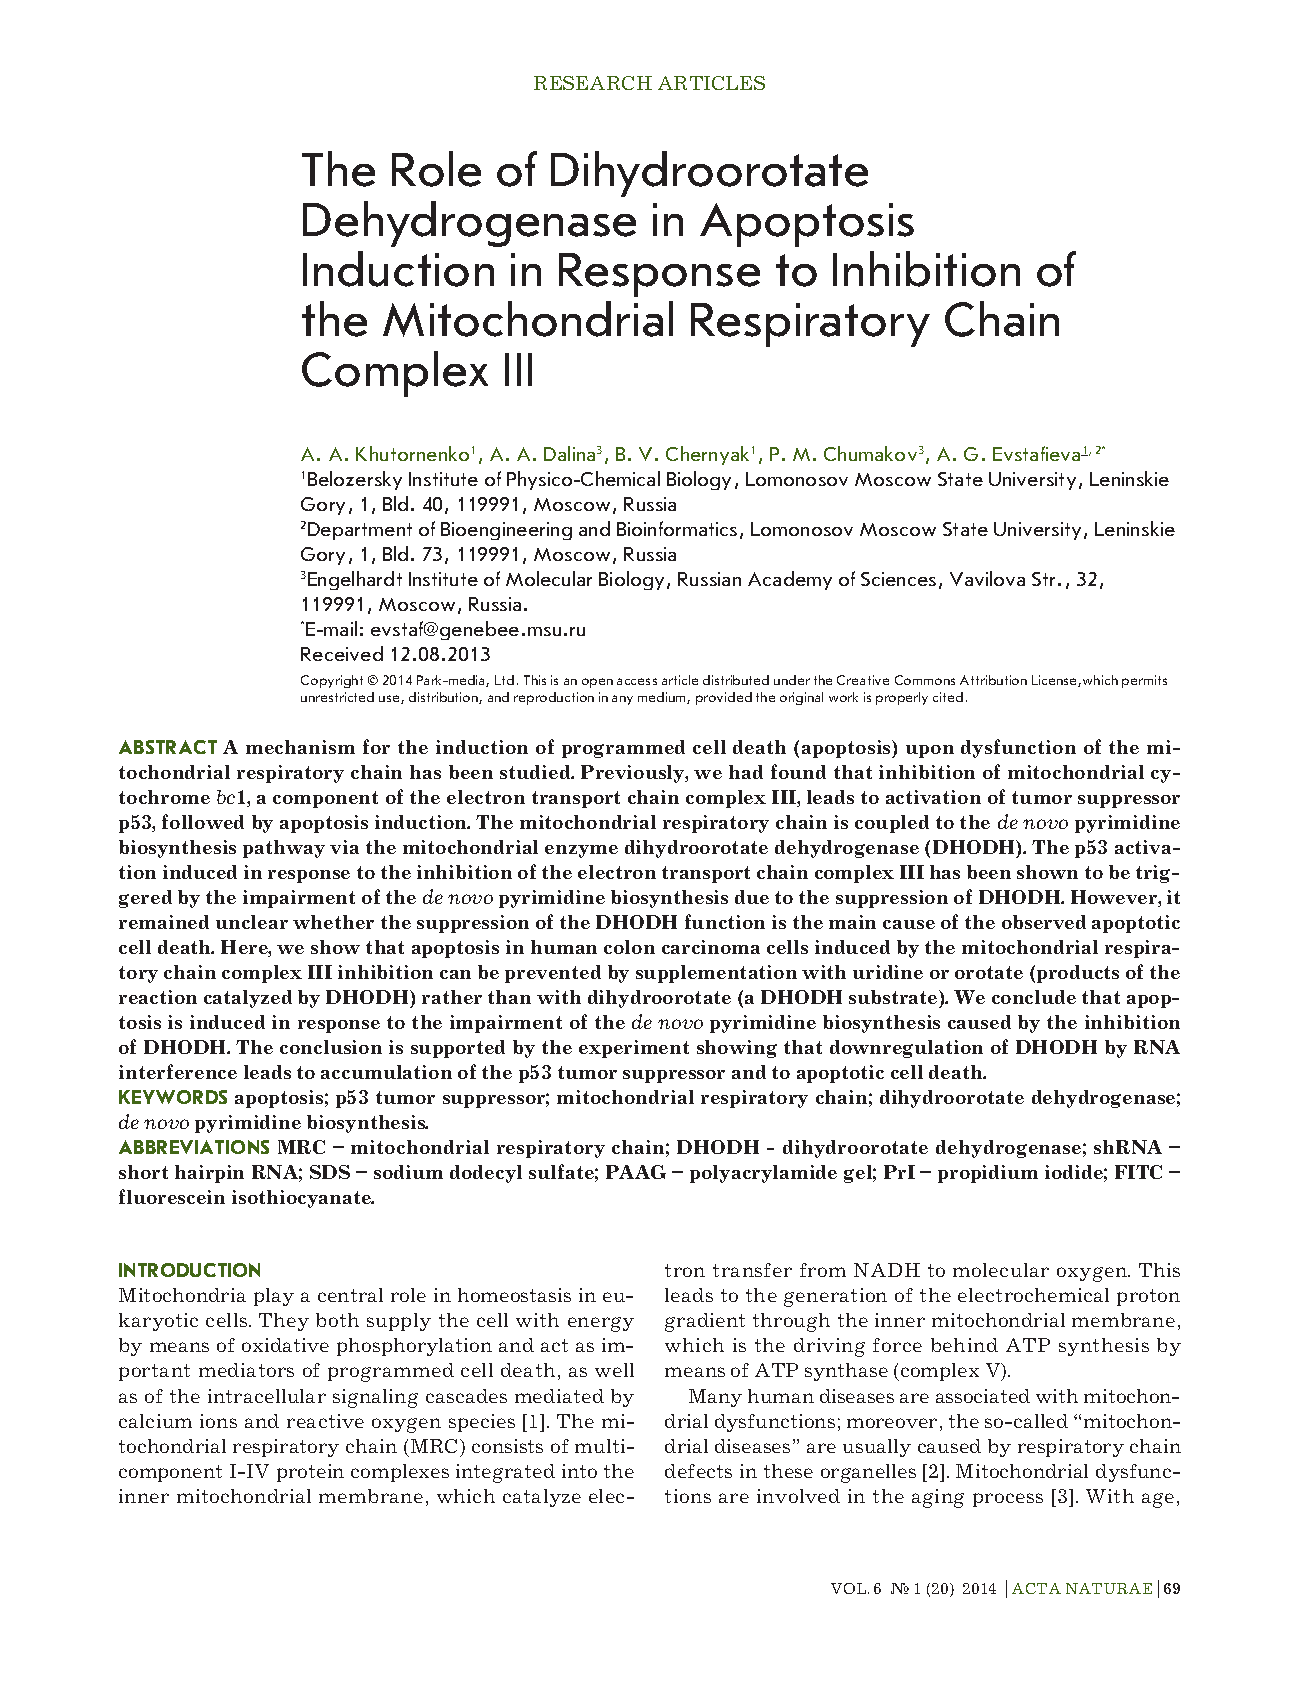
\includepdf[pages=-]{reading.pdf}
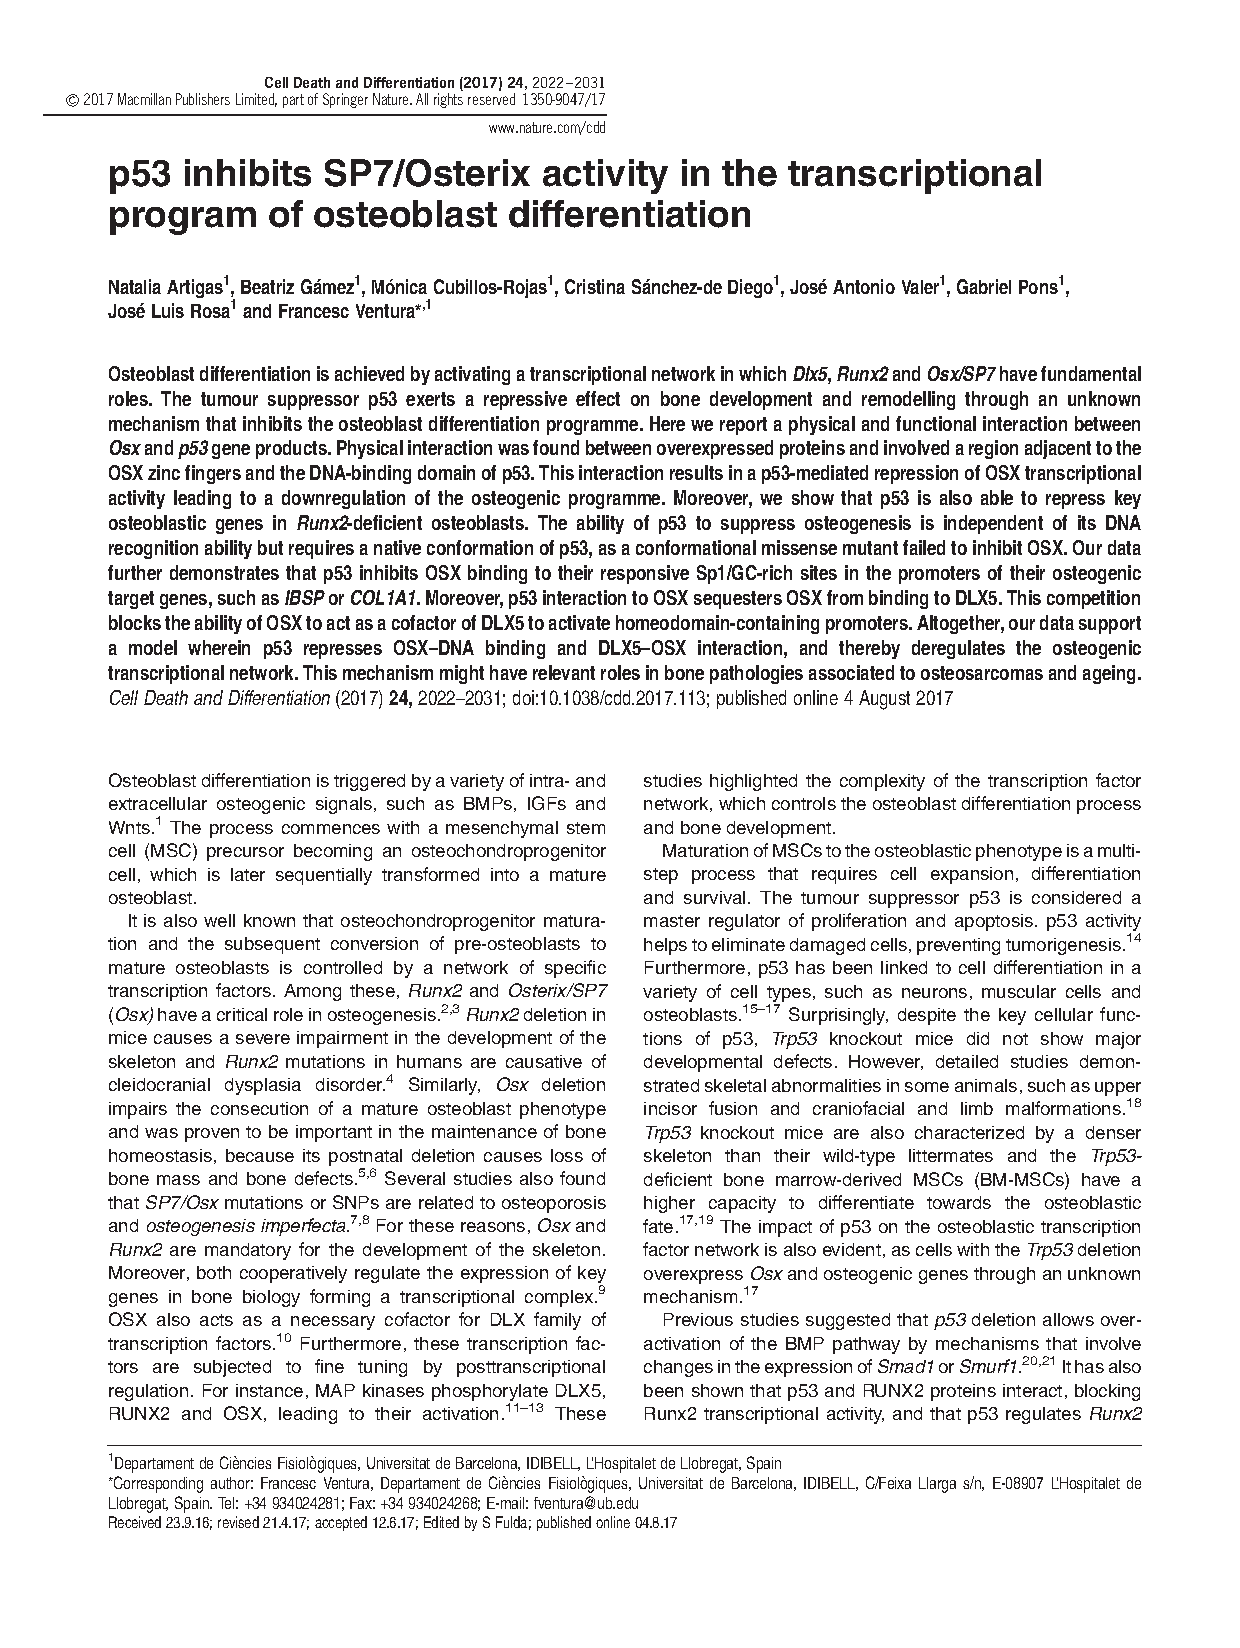
\includepdf[pages=-]{reading2.pdf}


\end{document}